\subsubsection{Klasifikasi Fungsional dan Semantik Smart Contracts}

\begin{figure}[ht]
	\centering
	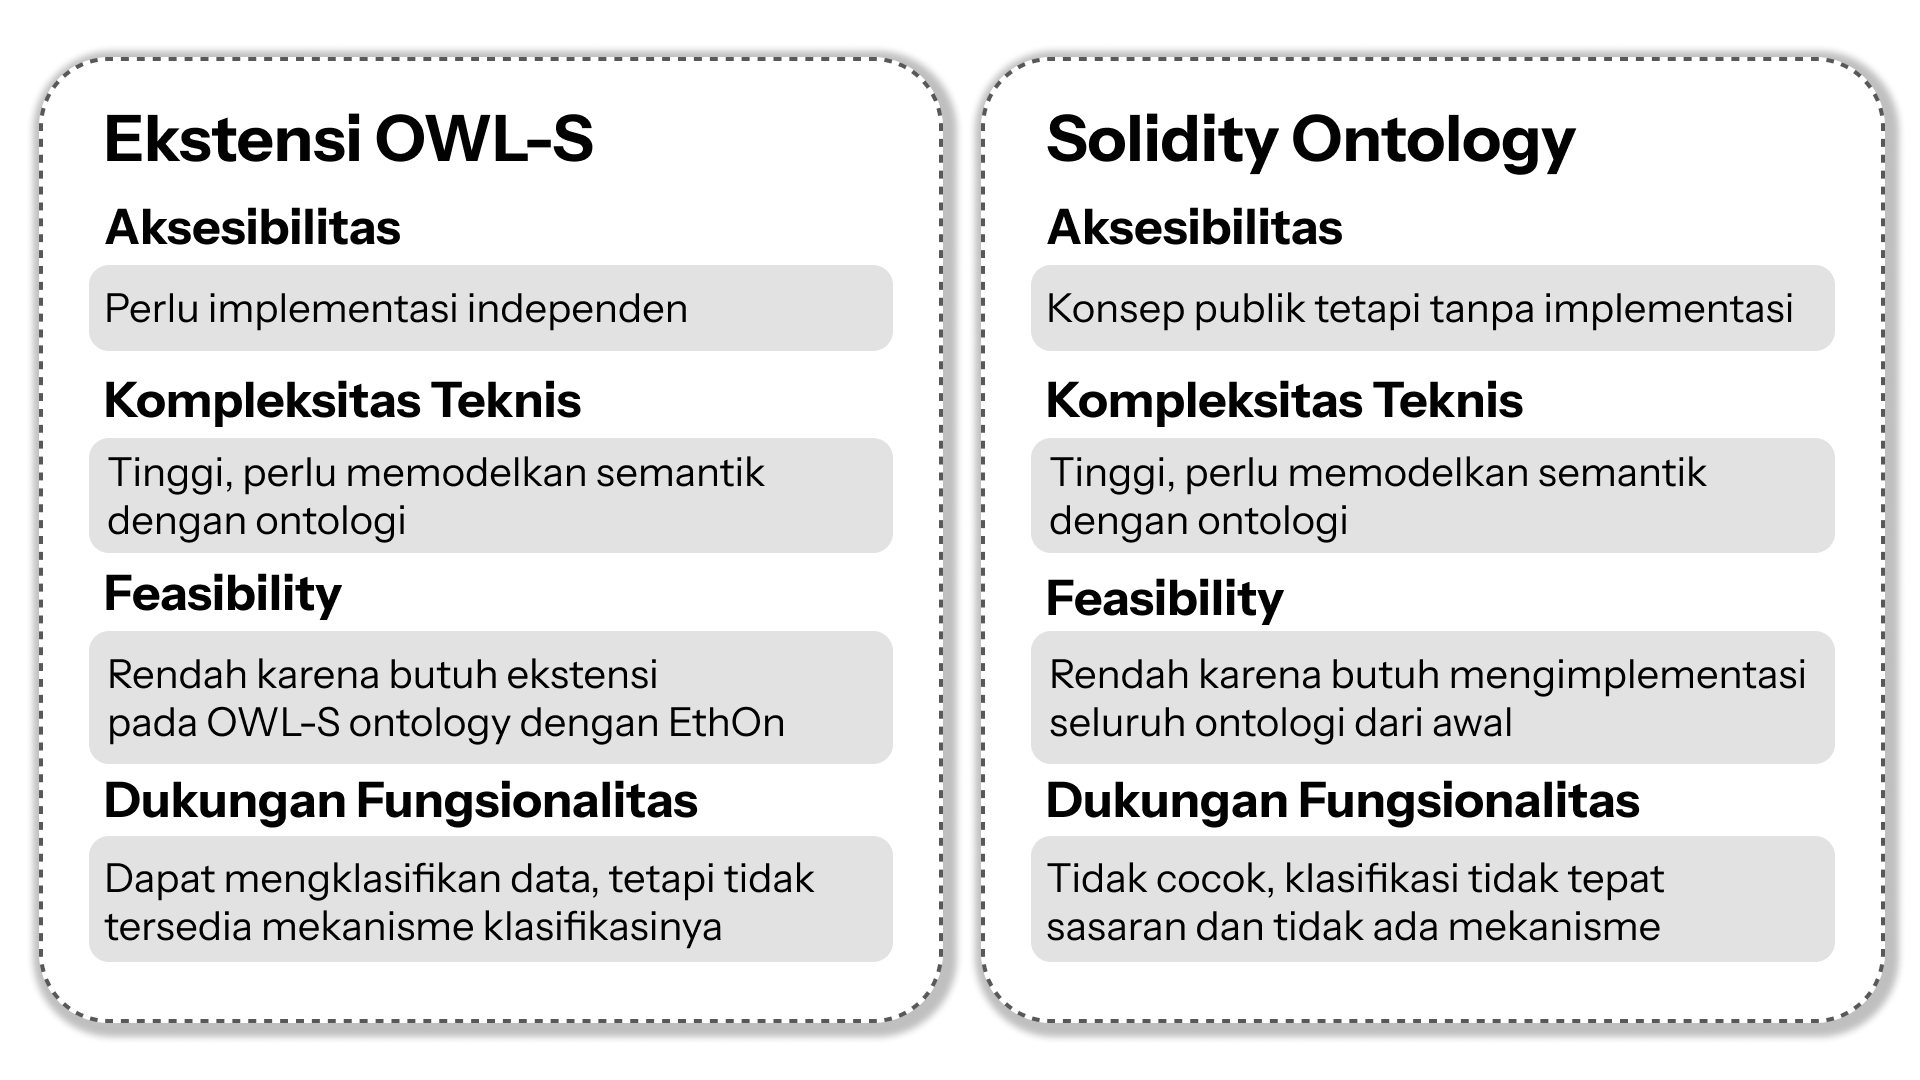
\includegraphics[width=0.7\textwidth]{resources/chapter-3/klasifikasi - 1.png}
	\caption{Perbandingan alternatif klasifikasi fungsional dan semantik Smart Contracts}
    \label{image:klasifikasi-1}
\end{figure}

\begin{figure}[ht]
	\centering
	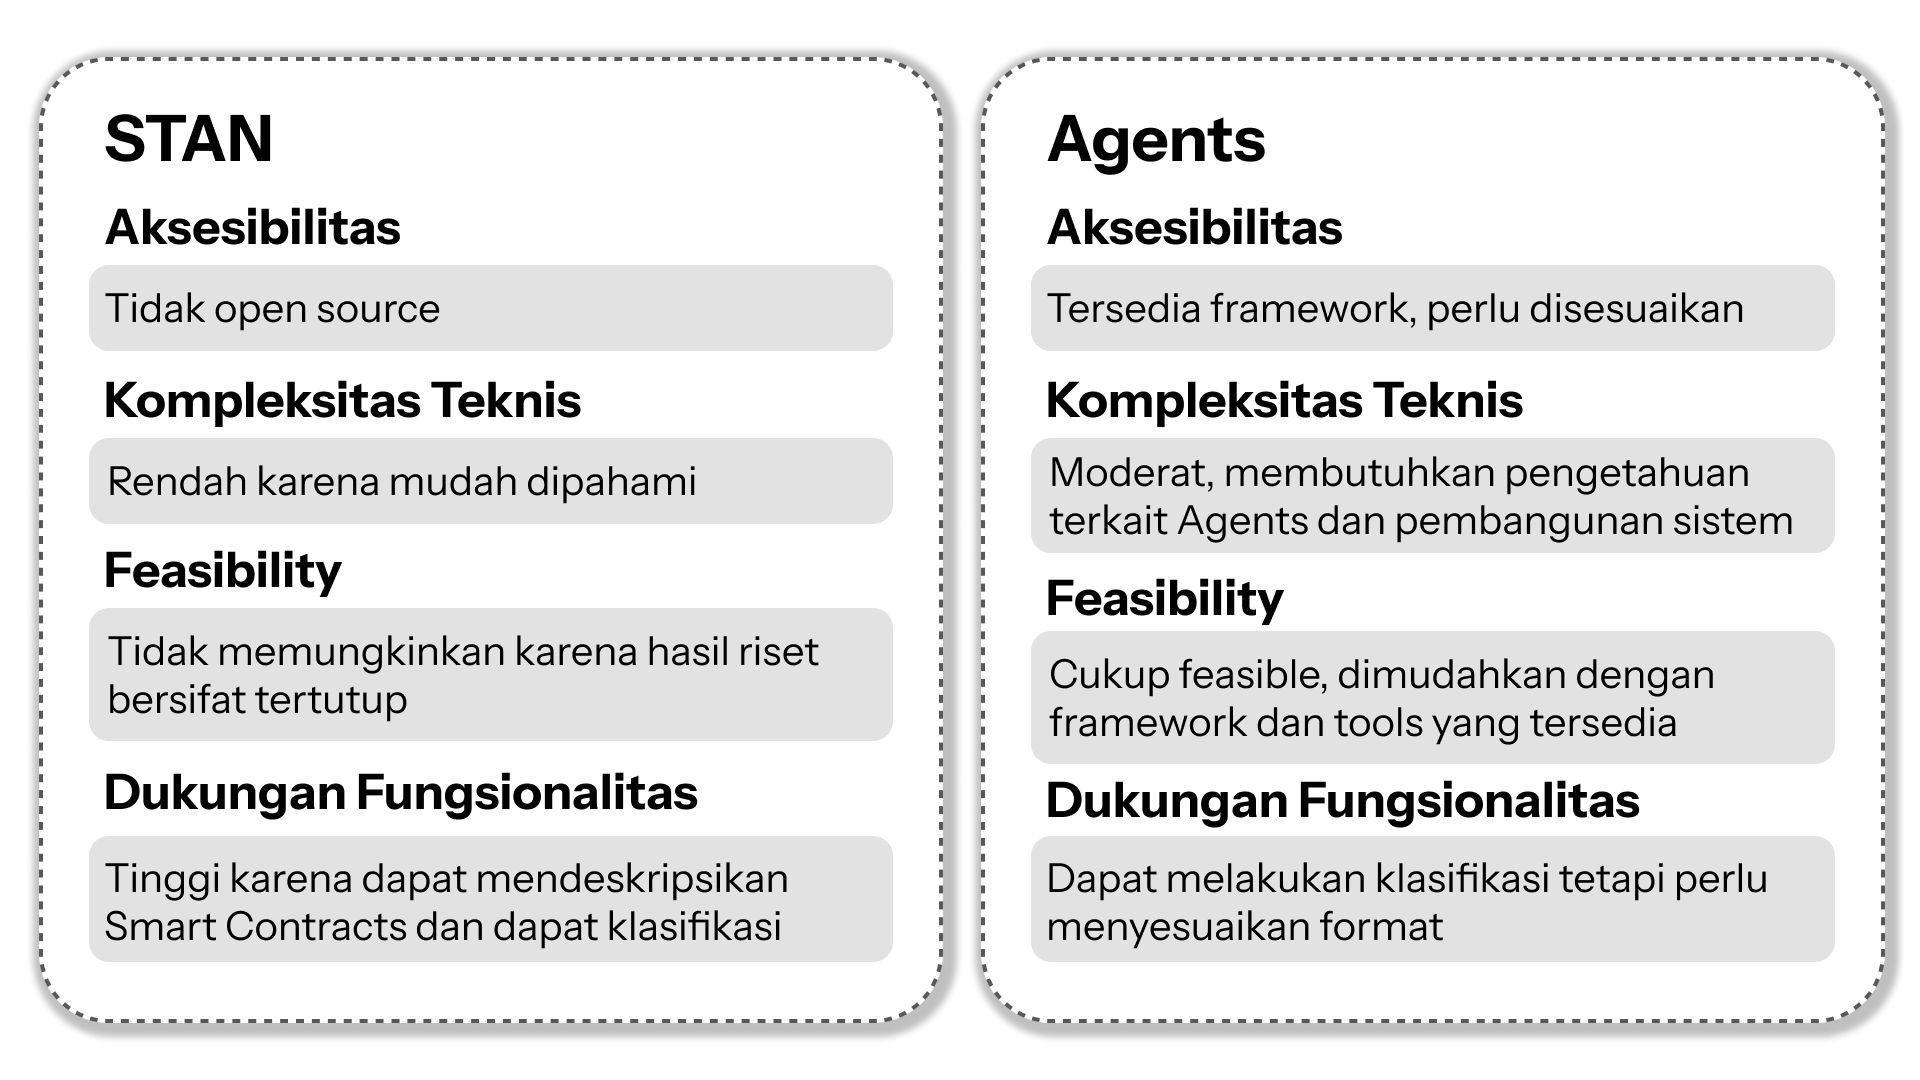
\includegraphics[width=0.7\textwidth]{resources/chapter-3/klasifikasi - 2.png}
	\caption{Perbandingan alternatif klasifikasi fungsional dan semantik Smart Contracts}
    \label{image:klasifikasi-2}
\end{figure}

\begin{figure}[ht]
	\centering
	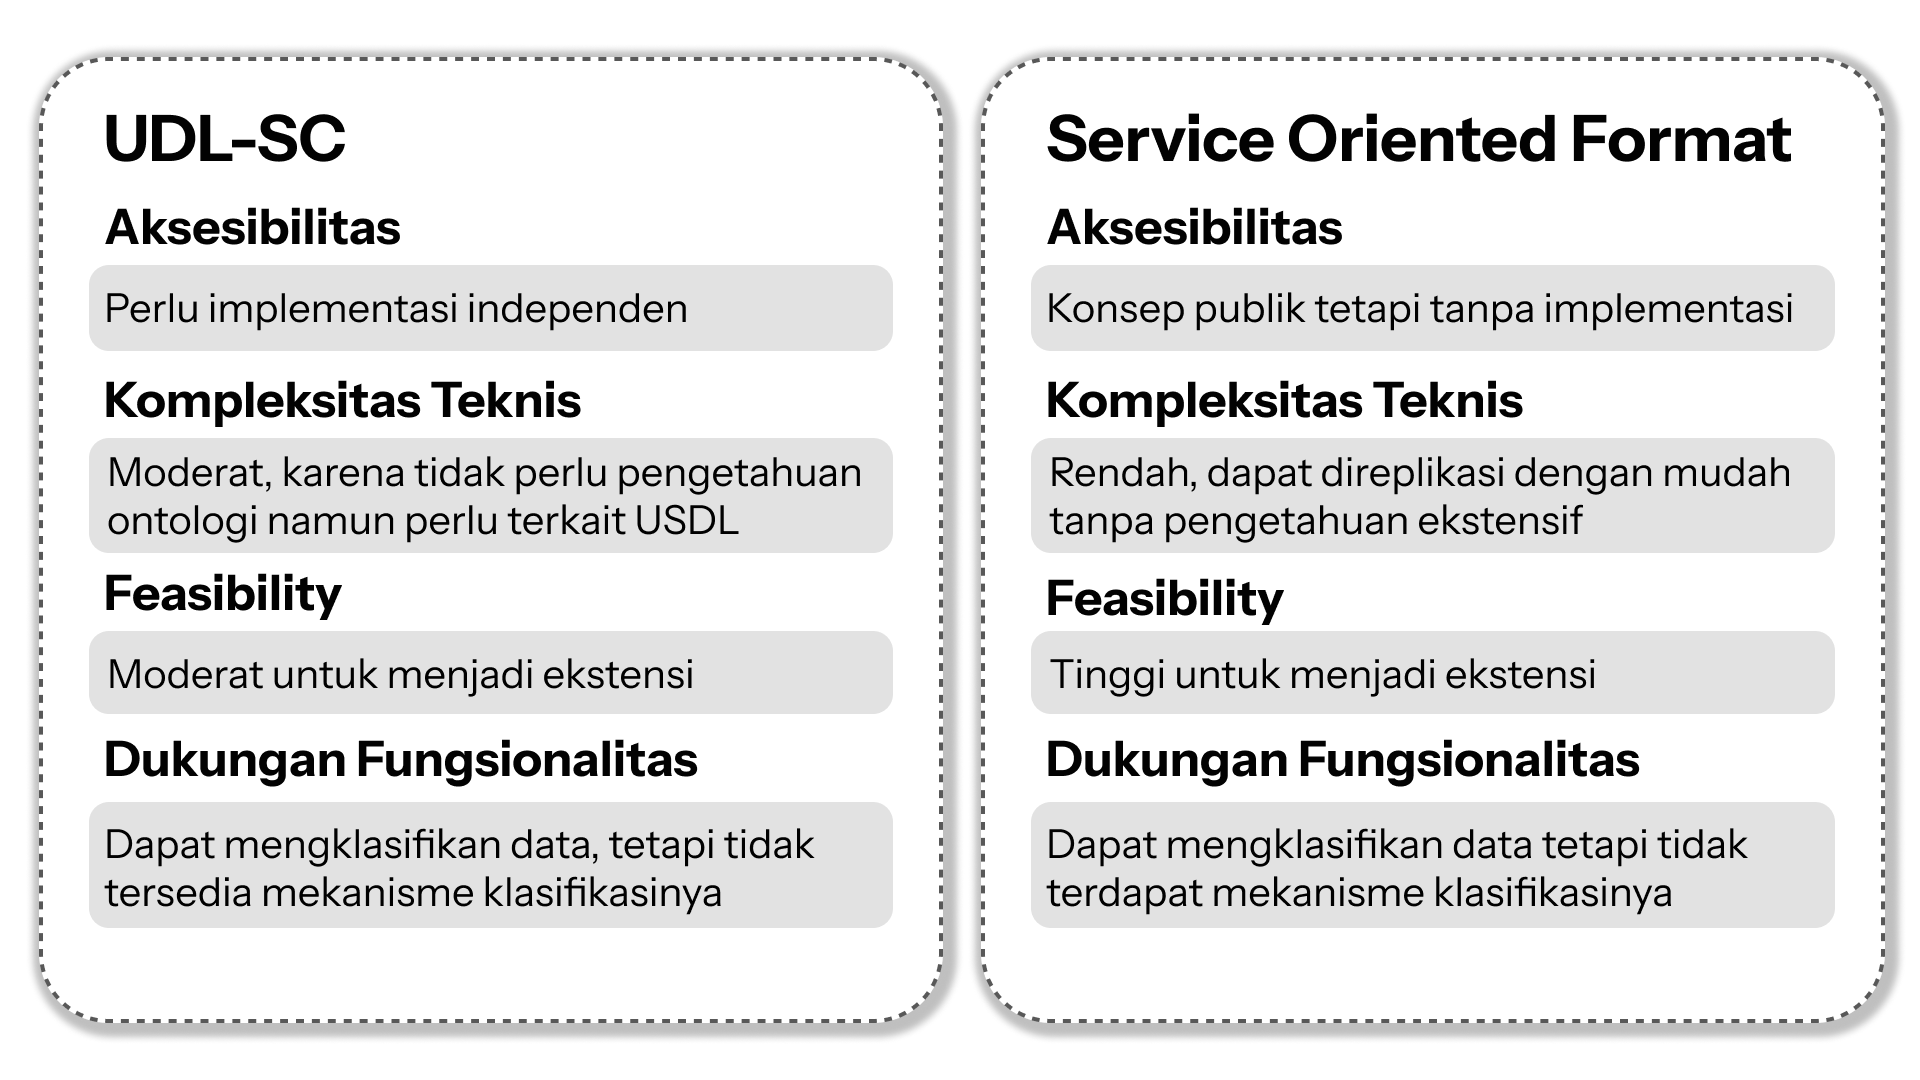
\includegraphics[width=0.7\textwidth]{resources/chapter-3/klasifikasi - 3.png}
	\caption{Perbandingan alternatif klasifikasi fungsional dan semantik Smart Contracts}
    \label{image:klasifikasi-3}
\end{figure}

\begin{figure}[ht]
	\centering
	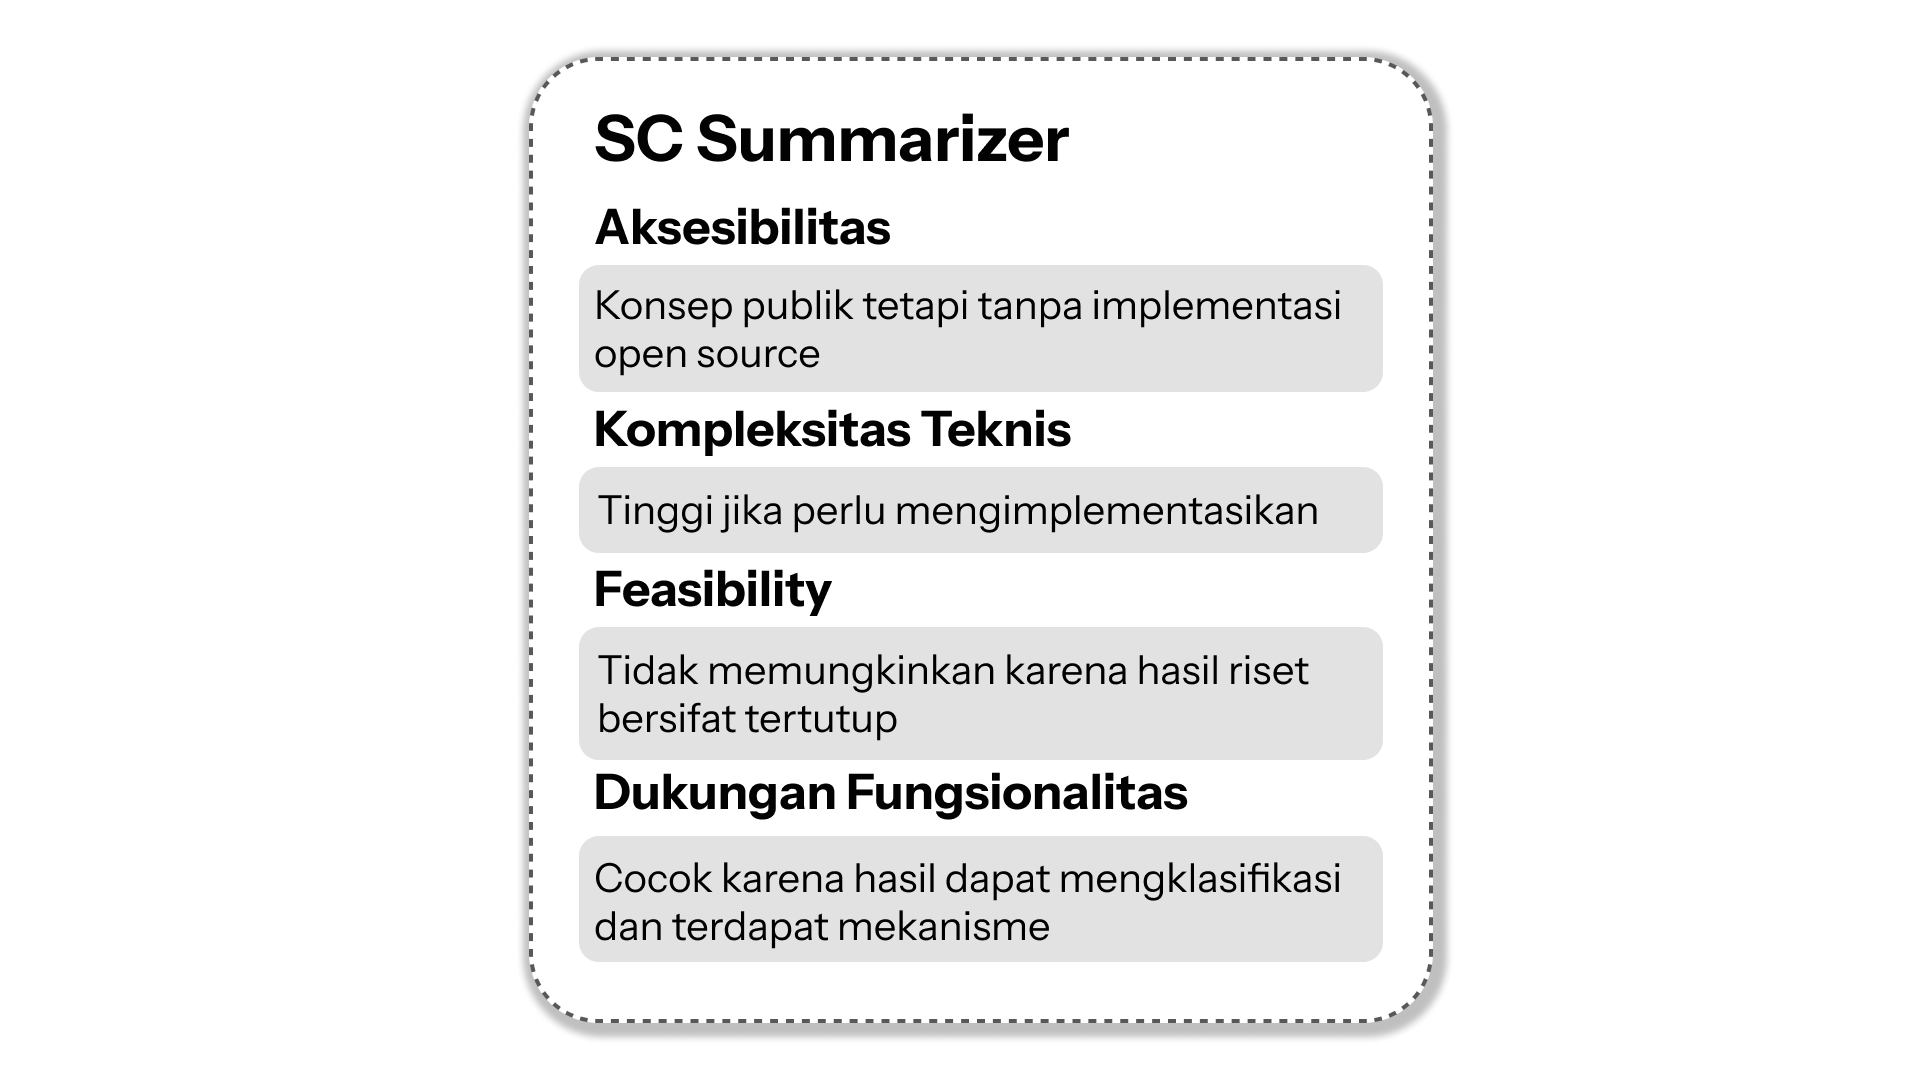
\includegraphics[width=0.7\textwidth]{resources/chapter-3/klasifikasi - 4.png}
	\caption{Perbandingan alternatif klasifikasi fungsional dan semantik Smart Contracts}
    \label{image:klasifikasi-4}
\end{figure}

Data yang sudah dimodelkan dan disimpan ke dalam sistem perlu dilakukan klasifikasi untuk memudahkan pencarian Smart Contracts berdasarkan fungsionalitas dan semantik. Terdapat berbagai alternatif untuk melakukan klasifikasi fungsional dan semantik Smart Contracts dengan berbagai pendekatan, baik dengan pemodelan ontologi, deskripsi fungsional, maupun format lainnya. Dukungan fungsional yang baik untuk klasifikasi adalah riset yang dapat melakukan klasifikasi pada data Smart Contracts dengan baik dan memberikan deskripsi atau hasil klasifikasi yang baik. Pada bagian ini, aspek skalabilitas digantikan dengan aspek \textit{feasibility}. Berikut adalah beberapa alternatif yang dapat digunakan untuk klasifikasi fungsional dan semantik Smart Contracts:

\begin{enumerate}
    \item \textbf{Semantic Smart Contracts for Blockchain-based Services in the Internet of Things} \parencite{baqa2019semantic} (Bagian \ref{subsec:semantic-smart-contract-iot}): Riset ini menggunakan ekstensi pada OWL-S Service Ontology untuk melakukan klasifikasi Smart Contracts berdasarkan semantik dan fungsionalitas. Keunggulannya adalah penggunaan ontologi yang dapat di-\textit{extend} untuk menambahkan terminologi yang \textit{domain specific}. Secara aksesibilitas, riset ini bersifat \textit{public}, namun tidak memiliki implementasi \textit{open source}. Selain itu, riset ini terbatas pada \textit{scope} Internet-of-Things. Secara kompleksitas, riset ini tergolong tinggi karena memerlukan pemahaman yang mendalam tentang ontologi dan pemodelan semantik. Dalam hal dukungan fungsional, riset ini dapat memberikan deskripsi yang baik, tetapi tidak terdapat mekanisme untuk mengklasifikasikan data dengan baik.
    
    \item \textbf{Ontological Modeling of Smart Contracts in Solidity} \parencite{cano2021toward} (Bagian \ref{subsec:solidity-ontology}): Riset ini menerapkan ontologi pada bahasa pemrograman Solidity. Ontologi ini digunakan untuk mendeskripsikan elemen-elemen dalam Smart Contracts, seperti fungsi, variabel, dan struktur data. Secara aksesibilitas, riset ini bersifat publik, dengan ontologi yang dihasilkan dapat diterapkan. Namun, implementasi ontologi pada riset ini terbatas pada sintaks dan semantik dari kode bahasa pemrograman Solidity sendiri dibandingkan Smart Contracts secara keseluruhan. Secara kompleksitas, riset ini tergolong tinggi karena memerlukan pemahaman yang mendalam tentang ontologi dan pemodelan semantik, dan memerlukan proses klasifikasi yang ekstensif untuk memetakan data dengan ontologi yang dihasilkan. Dalam hal dukungan fungsional, riset ini tidak sesuai dengan kebutuhan sistem, yaitu memodelkan fungsionalitas dari Smart Contract, bukan aspek sintaks bahasa pemrograman Soliditynya, dan tidak terdapat mekanisme untuk mengklasifikasikan data dengan baik.
    
    \item \textbf{STAN} \parencite{stan} (Bagian \ref{subsec:stan}): STAN adalah sebuah sistem untuk memberikan deskripsi terhadap bytecodes dari Smart Contracts. Secara aksesibilitas, STAN tidak bersifat \textit{open source}, sehingga tidak tersedia implementasinya untuk melakukan replikasi. Secara kompleksitas, STAN tergolong rendah karena abstraksi yang sudah diberikan untuk menghasilkan deskripsi. Riset STAN ini juga belum menginkorporasikan teknologi seperti Artificial Intelligence (AI) untuk melakukan klasifikasi. Dalam hal dukungan fungsional, STAN dapat membantu mengklasifikasikan Smart Contracts berdasarkan deskripsi yang dihasilkan.
    
    \item \textbf{Agents} (Bagian \ref{sec:agents}): Alternatif untuk melakukan klasifikasi Smart Contracts adalah menggunakan AI Agents yang dapat melakukan dekomposisi tasks yang kompleks menjadi sub-tasks yang lebih sederhana. Dengan menggunakan AI Agents, klasifikasi Smart Contracts dapat dilakukan dengan lebih menyeluruh dan efisien karena dapat memperhitungkan berbagai aspek yang ada pada Smart Contracts. Secara aksesibilitas, sudah banyak \textit{framework} dan \textit{tools} yang tersedia untuk membangun sebuah sistem berbasis AI Agents (Agentic AI). Namun, perlu dilakukan pembangunan secara independen karena tidak ada sistem yang secara langsung memberikan fungsionalitas yang sesuai. Secara kompleksitas, penggunaan AI Agents tergolong moderat karena memerlukan pengetahuan terkait AI dan membuat sistem berbasis AI Agents. Secara \textit{feasibility}, pembangunan sistem berbasis agents cukup \textit{feasible} dengan penggunaan \textit{framework} dan \textit{tools} yang baik. Dukungan fungsional yang diberikan oleh sistem dengan AI Agents tergolong baik karena dapat disesuaikan dan melakukan pekerjaan kompleks secara otonom, tetapi perlu menggunakan format yang disesuaikan untuk mendeskripsikan data.
    % menggunakan agents yang dimasukkin source code, dengan break down step by step

    \item \textbf{Uniform Description Language for Smart Contracts} \parencite{udlsc} (Bagian \ref{subsec:uniform-description-language}): Riset ini mengusulkan sebuah bahasa deskripsi ekstensi dari USDL untuk Smart Contracts. Secara aksesibilitas, hasil dari riset ini bersifat \textit{public}, namun perlu melakukan replikasi untuk mendapatkan hasil yang didapatkan dari riset. Secara kompleksitas, riset ini tergolong moderat karena walaupun tidak memerlukan pengetahuan yang mendalam terkait ontologi, perlu memahami terkait USDL dan implementasi ekstensi dari USDL. Secara skalabilitas, riset ini tergolong baik karena dapat digunakan sebagai ekstensi data tanpa masalah. Dalam hal dukungan fungsional, riset ini kurang baik karena tidak terdapat mekanisme untuk mengklasifikasikan data dengan baik, tetapi dapat digunakan untuk mendeskripsikan data Smart Contracts dengan baik.
    
    \item \textbf{Service Oriented Format Descriptor} \parencite{guida2019supporting} (Bagian \ref{subsec:supporting-reuse-smart-contracts}): Riset ini mengusulkan sebuah format deskripsi untuk Smart Contracts dengan pendekatan Service. Riset ini juga mengusulkan sebuah Service Registry dan Contract Editor berbasis visual yang mengkomplemen format deskripsi yang diusulkan. Format deskripsi ini dapat digunakan dan digabungkan dengan sistem lain, sedangkan Service Registry dan Contract Editor kurang fleksibel untuk diintegrasikan dengan sistem lain. Secara aksesibilitas, hasil dari riset ini bersifat \textit{public} dan \textit{open source}, sehingga dapat digunakan untuk melakukan replikasi. Secara kompleksitas, format yang dihasilkan oleh riset ini tergolong rendah karena tidak memerlukan pengetahuan yang mendalam dan dapat langsung dijadikan ekstensi ke format lain. Dalam hal dukungan fungsional, riset ini dapat mengakomodasi deskripsi Smart Contracts dengan baik, tetapi tidak ada mekanisme untuk melakukan klasifikasi data dengan baik.
    
    \item \textbf{Smart Contract Summarizer} \parencite{zhang2021smart} (Bagian \ref{subsec:smart-contract-solidity-summary}): Riset ini mengusulkan sebuah sistem untuk menghasilkan ringkasan dan anotasi dari Smart Contracts, terutama dalam bahasa Solidity. Sistem ini menggunakan teknik NLG (Natural Language Generation) dengan pendekatan berbasis \textit{transformer} untuk menghasilkan ringkasan yang lebih baik dibandingkan dengan metode berbasis template sebelumnya. Secara aksesibilitas, konsep dari riset ini bersifat \textit{public}, namun tidak memiliki implementasi \textit{open source}. Secara kompleksitas, jika perlu mengimplementasikan dari awal, riset ini tergolong tinggi karena memerlukan pengetahuan yang mendalam terkait NLP dan pemodelan semantik. Secara skalabilitas, sistem ini tidak diketahui untuk kinerja menangani data yang banyak. Dalam hal dukungan fungsional, riset ini dapat membantu mengklasifikasikan Smart Contracts berdasarkan ringkasan yang dihasilkan dengan mekanisme yang digunakan.

\end{enumerate}

Secara singkat, ketujuh alternatif ini dapat disimpulkan dengan diagram-diagram pada gambar \ref{image:klasifikasi-1}, gambar \ref{image:klasifikasi-2}, gambar \ref{image:klasifikasi-3}, dan gambar \ref{image:klasifikasi-4}.
